\section{初等变换与几何变换}

\subsection{初等变换}

\begin{definition}[矩阵的初等变换]
    矩阵的初等行变换与初等列变换统称为\textit{初等变换}. 下列三种关于矩阵的变换称为矩阵的\textit{初等行 (列) 变换}:
    \begin{enumerate}[label=(\arabic{*})]
        \item 互换矩阵中两行 (列) 的位置 $ \left(r_{i} \leftrightarrow r_{j}, c_{i} \leftrightarrow c_{j}\right)$ ;
        \item 以一非零常数乘矩阵的某一行 (列) $ \left(k r_{i}, k c_{j}\right) $;
        \item 将矩阵的某一行 (列) 的 $ k $ 倍加到另一行 (列) 上去 $ \left(r_{i}+k r_{j}, c_{i}+k c_{j}\right) $.
    \end{enumerate}
\end{definition}

\begin{example}
    设 $\vb*{A}=\mqty(\xmat*{a}{3}{3}),~\vb*{B}=\mqty(a_{21}&a_{22}&a_{23}\\a_{11}&a_{12}&a_{13}\\a_{31}+a_{11}&a_{32}+a_{12}&a_{33}+a_{13})$, 
    $$\vb*{P}_1=\mqty(0&1&0\\1&0&0\\0&0&1),~\vb*{P}_2=\mqty(1&0&0\\0&1&0\\1&0&1)$$
    则必有 (\quad).
    \begin{tasks}(4)
        \task $\vb*{AP}_1\vb*{P}_2=\vb*{B}$
        \task $\vb*{AP}_2\vb*{P}_1=\vb*{B}$
        \task $\vb*{P}_1\vb*{P}_2\vb*{A}=\vb*{B}$
        \task $\vb*{P}_2\vb*{P}_1\vb*{A}=\vb*{B}$
    \end{tasks}
\end{example}
\begin{solution}
    矩阵 $\vb*{B}$ 是矩阵 $\vb*{A}$ 经过初等行变换得到的, 首先把矩阵 $\vb*{A}$ 的第一行加到第三行, 即 $\vb*{P}_2\vb*{A}$;
    然后再把 $\vb*{P}_2\vb*{A}$ 的第一行与第二行互换, 即选 C.
\end{solution}

\begin{example}
    设 $\vb*{A}$ 是 3 阶方阵, 将 $\vb*{A}$ 的第 1 列与第 2 列交换得到 $\vb*{B}$, 再把 $\vb*{B}$ 的第 2 列加到第 3 列 得到 $\vb*{C}$, 求满足 $\vb*{AQ}=\vb*{C}$ 的可逆矩阵 $\vb*{Q}$.
\end{example}
\begin{solution}
    将所述变换用相应的初等矩阵表示, 即 $\vb*{B}=\vb*{AE}_{12}$, $\vb*{C}=\vb*{BE}_{23}(1)$, 那么 $\vb*{C}=\vb*{AE}_{12}\vb*{E}_{23}(1)$, 则
    $$\vb*{Q}=\vb*{E}_{12}\vb*{E}_{23}(1)=\mqty(0&1&0\\1&0&0\\0&0&1)\mqty(1&0&0\\0&1&1\\0&0&1)=\mqty(0&1&1\\1&0&0\\0&0&1).$$
\end{solution}

\begin{example}
    设 $\vb*{A}=\mqty(1&2&3\\4&5&6\\7&8&9),~\vb*{P}=\mqty(\admat{1,1,1}),~\vb*{Q}=\mqty(1&&\\&&1\\&1&)$, 求 $\vb*{P}^{2022}\vb*{AQ}^{2023}.$
\end{example}
\begin{solution}
    $\vb*{P}$ 左乘 $\vb*{A}$ 相当于把 $\vb*{A}$ 的第 1、3 行互换, 故 $\vb*{P}^{2022}\vb*{A}$ 是把 $\vb*{A}$ 的第 1、3 行互换 2022 次, 结果仍为 $\vb*{A}$;
    同理 $\vb*{AQ}^{2023}$ 相当于把 $\vb*{A}$ 的第 2、3 列互换 2023 次, 那么结果为 $\mqty(1&3&2\\4&6&5\\7&9&8).$
\end{solution}

\begin{example}[2006 数一]
    设 $\vb*{A}$ 为 3 阶方阵, 将 $\vb*{A}$ 的第 2 行加到第 1 行得 $\vb*{B}$, 再将 $\vb*{B}$ 的第 1 列的 -1 倍加到第 2 列得 $\vb*{C}$, 记 $\vb*{P}=\mqty(1&1&0\\0&1&0\\0&0&1)$, 则有
    \begin{tasks}(4)
        \task $\vb*{C}=\vb*{P}^{-1}\vb*{AP}$
        \task $\vb*{C}=\vb*{PAP}^{-1}$
        \task $\vb*{C}=\vb*{P}^\top\vb*{AP}$
        \task $\vb*{C}=\vb*{PAP}^\top$
    \end{tasks}
\end{example}
\begin{solution}
    将所述变换用相应的初等矩阵表示, $\vb*{B}=\vb*{E}_{12}(1)\vb*{A},~\vb*{C}=\vb*{BE}_{12}(-1)$, 于是 $$\vb*{C}=\vb*{E}_{12}(1)\vb*{A}\vb*{E}_{23}(1)=\vb*{PAP}^{-1}$$
    故选 B.
\end{solution}

\begin{example}[2009 数二]
    设 $\vb*{A},~\vb*{P}$ 均为 3 阶方阵, 且 $\vb*{P}^\top\vb*{AP}=\mqty(1&0&0\\0&1&0\\0&0&2)$, 若 $\vb*{P}=(\vb*{\alpha}_1,\vb*{\alpha}_2,\vb*{\alpha}_3)$, $\vb*{Q}=(\vb*{\alpha}_1+\vb*{\alpha}_2,\vb*{\alpha}_2,\vb*{\alpha}_3)$, 
    则 $\vb*{Q}^\top\vb*{AQ}$ 为 (\quad).
    \begin{tasks}(4)
        \task $\mqty(2&1&0\\1&1&0\\0&0&2)$
        \task $\mqty(1&1&0\\1&2&0\\0&0&2)$
        \task $\mqty(2&0&0\\0&1&0\\0&0&2)$
        \task $\mqty(1&0&0\\0&2&0\\0&0&2)$
    \end{tasks}
\end{example}
\begin{solution}
    由题意, $\vb*{Q}=\vb*{PE}_{21}(1)$, 那么
    \begin{flalign*}
        \vb*{Q}^\top\vb*{AQ} & =\qty(\vb*{PE}_{21}(1))^\top\vb*{APE}_{21}(1)=\vb*{E}_{21}^\top(1)\vb*{P}^\top\vb*{APE}_{21}(1)         \\
                             & =\mqty(1                                                                                        & 1 & 0 \\0&1&0\\0&0&1)\mqty(1&0&0\\0&1&0\\0&0&2)\mqty(1&0&0\\1&1&0\\0&0&1)=\mqty(2&1&0\\1&1&0\\0&0&2)
    \end{flalign*}
    故选 A.
\end{solution}

\begin{example}
    (2021 数二) 已知矩阵 $\vb*{A}=\begin{pmatrix}
            1  & 0  & -1 \\
            2  & -1 & 1  \\
            -1 & 2  & -5
        \end{pmatrix}$, 若存在下三角可逆矩阵 $\vb*{P}$ 和上三角可逆矩阵 $\vb*{Q}$,
    使 $\vb*{PAQ}$ 为对角矩阵, 求 $\vb*{P}$ 和 $\vb*{Q}$.
\end{example}
\begin{solution}
    对 $\vb*{A}$ 作初等行变换, 化为上三角矩阵 $\vb*{B}$,
    \begin{flalign*}
        \begin{pNiceArray}{c:c}
            \vb*{A} & \vb*{E}
        \end{pNiceArray} & =\begin{pNiceArray}{ccc:ccc}
                                1  & 0  & -1 & 1 & 0 & 0 \\
                                2  & -1 & 1  & 0 & 1 & 0 \\
                                -1 & 2  & -5 & 0 & 0 & 1 \\
                            \end{pNiceArray}\xrightarrow[r_3+r_1]{r_2-2r_1}
        \begin{pNiceArray}{ccc:ccc}
            1 & 0  & -1 & 1  & 0 & 0 \\
            0 & -1 & 3  & -2 & 1 & 0 \\
            0 & 2  & -6 & 1  & 0 & 1 \\
        \end{pNiceArray}                                                   \\
                                & \xrightarrow[]{r_3+2r_2}\begin{pNiceArray}{ccc:ccc}
                                                              1 & 0  & -1 & 1  & 0 & 0 \\
                                                              0 & -1 & 3  & -2 & 1 & 0 \\
                                                              0 & 0  & 0  & -3 & 2 & 1 \\
                                                          \end{pNiceArray}
        \xrightarrow[]{}\begin{pNiceArray}{ccc:ccc}
                            1 & 0 & -1 & 1  & 0  & 0 \\
                            0 & 1 & -3 & 2  & -1 & 0 \\
                            0 & 0 & 0  & -3 & 2  & 1 \\
                        \end{pNiceArray}=\begin{pNiceArray}{c:c}
                                             \vb*{B} & \vb*{P}
                                         \end{pNiceArray}
    \end{flalign*}
    所以 $\vb*{P}=\begin{pmatrix}
            1  & 0  & 0 \\
            2  & -1 & 0 \\
            -3 & 2  & 1
        \end{pmatrix}$, 再对 $\vb*{B}$ 作列变换 (或 $\vb*{B}^{\top}$ 作行变换) 化为对角矩阵, 可求得 $\vb*{Q}$ (或 $\vb*{Q}^{\top}$)
    $$\begin{pNiceArray}{c}
            \vb*{B} \\
            \hdottedline
            \vb*{E}
        \end{pNiceArray}=\begin{pNiceArray}{ccc}
            1 & 0 & -1 \\
            0 & 1 & -3 \\
            0 & 0 & 0  \\
            \hdottedline
            1 & 0 & 0  \\
            0 & 1 & 0  \\
            0 & 0 & 1
        \end{pNiceArray}\xrightarrow[c_3+3c_1]{c_3+c_1}\begin{pNiceArray}{ccc}
            1 & 0 & 0 \\
            0 & 1 & 0 \\
            0 & 0 & 0 \\
            \hdottedline
            1 & 0 & 1 \\
            0 & 1 & 3 \\
            0 & 0 & 1
        \end{pNiceArray}$$
    可得 $\vb*{Q}=\begin{pmatrix}
            1 & 0 & 1 \\
            0 & 1 & 3 \\
            0 & 0 & 1
        \end{pmatrix}.$
    或 $$\begin{pNiceArray}{c:c}
            \vb*{B}^{\top} & \vb*{E}
        \end{pNiceArray}=\begin{pNiceArray}{ccc:ccc}
            1  & 0  & 0 & 1 & 0 & 0 \\
            0  & 1  & 0 & 0 & 1 & 0 \\
            -1 & -3 & 0 & 0 & 0 & 1 \\
        \end{pNiceArray}\xrightarrow[r_3+r_1]{r_3+3r_2}
        \begin{pNiceArray}{ccc:ccc}
            1 & 0 & 0 & 1 & 0 & 0 \\
            0 & 1 & 0 & 0 & 1 & 0 \\
            0 & 0 & 0 & 1 & 3 & 1 \\
        \end{pNiceArray}$$
    得 $\vb*{Q}^{\top}=\begin{pmatrix}
            1 & 0 & 0 \\
            0 & 1 & 0 \\
            1 & 3 & 1
        \end{pmatrix}.$
\end{solution}

\subsection{初等矩阵}

\begin{definition}[初等矩阵]
    由于初等变换有 3 种, 相应可以得到 3 种初等矩阵:
    \begin{enumerate}[label=(\arabic{*})]
        \item $\vb*{E}_{i j} \Leftrightarrow $ 交换 $ \vb*{E} $ 的第 $ i, j $ 两行 (或列) 所得到的矩阵;
        \item $\vb*{E}_{i}(k) \Leftrightarrow \vb*{E} $ 的第 $ i $ 行 (或列) 乘以非零常数 $ k $ 所得到的矩阵;
        \item $\vb*{E}_{i j}(k) \Leftrightarrow $ 把 $ \vb*{E} $ 的第 $ j $ 行的 $ k $ 倍加到第 $ i $ 行或者把 $ \vb*{E} $ 的第 $ i $ 列的 $ k $ 倍加到第 $ j $ 列所得到的矩阵.
    \end{enumerate}
\end{definition}

\begin{theorem}[初等矩阵的逆]
    \begin{enumerate*}[label=(\arabic{*})]
        \item $\vb*{E}_{ij}^{-1}=\vb*{E}_{ij}$;
        \item $\vb*{E}_i^{-1}(k)=\vb*{E}_i\qty(\dfrac{1}{k})$;
        \item $\vb*{E}_{ij}^{-1}(k)=\vb*{E}_{ij}(-k)$.
    \end{enumerate*}
\end{theorem}

\begin{theorem}[初等矩阵的幂]
    对于初等矩阵 $\vb*{E}_{ij}$ 的幂有公式: $\vb*{E}_{ij}^{n}=\begin{cases}
        \vb*{E},& n=2k\\ 
        \vb*{E}_{ij},& n=2k+1\\ 
    \end{cases}k\in \mathbb{N}.$
\end{theorem}

\begin{theorem}[初等变换与初等矩阵的联系]
    设 $\vb*{A}$ 是 $m\times n$ 矩阵, 对 $\vb*{A}$ 施行一次初等行变换, 相当于在 $\vb*{A}$ 的左边乘以相应的 $m$ 阶初等矩阵;
    对 $\vb*{A}$ 施行一次初等列变换, 相当于在 $\vb*{A}$ 的右边乘以相应的 $n$ 阶初等矩阵.
\end{theorem}

\begin{example}
    试将矩阵 $\mqty(2&3\\3&5)$ 写成若干个形如 $\mqty(1&0\\x&1)$ 与 $\mqty(1&y\\0&1)$ 的矩阵的乘积.
\end{example}
\begin{solution}
    显然, 所给矩阵非奇异, 故可经一系列初等变换化为单位矩阵, 具体地, 有
    $$\mqty(2&3\\3&5)\xrightarrow[c_2-c_1]{r_2-r_1}\mqty(2&1\\1&1)\xrightarrow[c_2-c_1]{c_1-c_2}\mqty(1&0\\0&1)$$
    用初等矩阵表示, 即
    $$\vb*{E}_{21}(-1)\mqty(2&3\\3&5)\vb*{E}_{12}(-1)\vb*{E}_{21}(-1)\vb*{E}_{12}(-1)=\mqty(1&0\\0&1)$$
    因此, 有
    \begin{flalign*}
        \mqty(2 & 3 \\3&5)=\vb*{E}_{21}^{-1}(-1)\vb*{E}_{12}^{-1}(-1)\vb*{E}_{21}^{-1}(-1)\vb*{E}_{12}^{-1}(-1)=\mqty(1&0\\1&1)\mqty(1&1\\0&1)\mqty(1&0\\1&1)\mqty(1&1\\0&1)
    \end{flalign*}
\end{solution}

\begin{example}
    设 $a\neq0$, 把矩阵 $\mqty(a&0\\0&a^{-1})$ 表示成一些形如 $\mqty(1&x\\0&1)$ 与 $\mqty(1&0\\y&1)$ 的矩阵的乘积.
\end{example}
\begin{solution}
    考虑如何用消法变换将 $\mqty(a&0\\0&a^{-1})$ 化为单位矩阵, 
    $$\mqty(a&0\\0&a^{-1})\xrightarrow[r_1+\frac{1-a}{a}r_2]{r_2+r_1}\mqty(1&\dfrac{1-a}{a^2}\\[6pt]a&a^{-1})\xrightarrow[r_1+\frac{a-1}{a^2}r_2]{r_2-ar_1}\mqty(1&0\\0&1)$$
    将上述过程用初等矩阵表示, 得
    \begin{flalign*}
        \vb*{E}_{12}\qty(\dfrac{a-1}{a^2})\vb*{E}_{21}(-a)\vb*{E}_{12}\qty(\dfrac{1-a}{a^2})\vb*{E}_{21}(1)\mqty(a & 0 \\0&a^{-1})=\mqty(1&0\\0&1)
    \end{flalign*}
    因此, 有
    \begin{flalign*}
        \mqty(a & 0 \\0&a^{-1})&=\vb*{E}_{21}^{-1}(1)\vb*{E}_{12}^{-1}\qty(\dfrac{1-a}{a^2})\vb*{E}_{21}^{-1}(-a)\vb*{E}_{12}^{-1}\qty(\dfrac{a-1}{a^2})=\mqty(1 & 0 \\-1&1)\mqty(1&\dfrac{a-1}{a}\\[6pt]0&1)\mqty(1&0\\a&1)\mqty(1&\dfrac{1-a}{a^2}\\[6pt]0&1)
    \end{flalign*}
\end{solution}

\begin{example}
    设矩阵 $\vb*{A}=\mqty(1&0&2\\1&-1&0\\0&1&2)$ 经初等行变换变为矩阵 $\vb*{B}=\mqty(-1&2&2\\2&-1&2\\-2&2&a)$
    \begin{enumerate}[label=(\arabic{*})]
        \item 求 $a$ 的值;
        \item 求满足 $\vb*{PA}=\vb*{B}$ 的所有可逆矩阵 $\vb*{P}.$
    \end{enumerate}
\end{example}
\begin{solution}
    \begin{enumerate}[label=(\arabic{*})]
        \item 易得 $\rank\vb*{A}=2$, 并且 $\vb*{B}=\mqty(-1&2&2\\2&-1&2\\-2&2&a)\xrightarrow[\substack{r_2\times\frac{1}{3}\\r_3-r_2}]{\substack{r_2+2r_1\\r_3+r_2}}\mqty(-1&2&2\\0&1&2\\0&0&a)$, 则 $\rank\vb*{B}=2\Rightarrow a=0$.
        \item 记 $\vb*{X}=(\vb*{x}_1,\vb*{x}_2,\vb*{x}_3),~\vb*{B}^\top=(\vb*{\beta}_1,\vb*{\beta}_2,\vb*{\beta}_3)$, 求解 $\vb*{A}^\top\vb*{X}=\vb*{B}^\top$, 转化为求解三个方程组 $\vb*{A}^\top\vb*{x}_i=\vb*{\beta}_i~~(i=1,2,3)$, 于是
              $$\begin{pNiceArray}{c|c}
                      \vb*{A}^\top&\vb*{B}^\top
                  \end{pNiceArray}=\begin{pNiceArray}{ccc|ccc}
                      1&0&2&-1&2&2\\
                      1&-1&0&2&-1&2\\
                      0&1&2&-2&2&0
                  \end{pNiceArray}\xrightarrow[r_1-r_2]{r_3-2r_1-2r_2}\begin{pNiceArray}{ccc|ccc}
                      1&0&1&\textcolor{cyan}{1}&  \textcolor{magenta}{1}&\textcolor{orange}{0}\\
                      0&1&-1&\textcolor{cyan}{-2}&\textcolor{magenta}{1}&\textcolor{orange}{-2}\\
                      0&0&0&\textcolor{cyan}{0}&  \textcolor{magenta}{0}&\textcolor{orange}{0}
                  \end{pNiceArray}$$
              因此 $\vb*{A}^\top\vb*{X}=\vb*{0}$ 的基础解系为 $\vb*{\xi}=\mqty(-1\\1\\1)$, 
              $\vb*{A}^\top\vb*{x}_i=\vb*{\beta}_i$ 的通解分别为
              \begin{flalign*}
                  \vb*{\eta}_1=k_1\vb*{\xi}+\mqty(\textcolor{cyan}{1}    \\\textcolor{cyan}{-2}\\\textcolor{cyan}{0})=\mqty(1-k_1\\-2+k_1\\k_1),~
                  \vb*{\eta}_2=k_2\vb*{\xi}+\mqty(\textcolor{magenta}{1} \\
                  \textcolor{magenta}{1}                                 \\
                  \textcolor{magenta}{0})=\mqty(1-k_2                    \\1+k_2\\k_2),~
                  \vb*{\eta}_3=k_3\vb*{\xi}+\mqty(\textcolor{orange}{0}  \\
                  \textcolor{orange}{-2}                                 \\
                  \textcolor{orange}{0})=\mqty(-k_3                      \\-2+k_3\\k_3)
              \end{flalign*}
              故满足 $\vb*{A}^\top\vb*{X}=\vb*{B}^\top$ 的解为
              $\vb*{X}\mqty(\vb*{\eta}_1,\vb*{\eta}_2,\vb*{\eta}_3)$, 当 $\det\vb*{X}\neq0$ 时, $\vb*{X}$ 可逆, 即
              $$\mqty|1-k_1&1-k_2&-k_3\\-2+k_1&1+k_2&-2+k_3\\k_1&k_2&k_3|=\mqty|1&1&0\\-2&1&-2\\k_1&k_2&k_3|=-2k_1+2k_2+3k_3\neq0.$$
    \end{enumerate}
\end{solution}

\begin{example}
    设矩阵 $$\vb*{A}=\mqty(1&0&0&2\\0&0&0&1\\-3&0&0&0)$$
    求三阶可逆矩阵 $\vb*{P}$, 四阶可逆矩阵 $\vb*{Q}$, 使得 $\vb*{A}=\vb*{P}\mqty(1&0&0&0\\0&1&0&0\\0&0&0&0)\vb*{Q}.$
\end{example}
\begin{solution}
    先对 $\vb*{A}$ 作初等变换, 有
    $$\vb*{A}\xrightarrow[\substack{r_3+3r_1\\c_2\leftrightarrow c_4}]{r_1-2r_2}\mqty(1&0&0&0\\0&1&0&0\\0&0&0&0)$$
    对应的初等矩阵为
    $$\vb*{E}_{31}(3)\vb*{E}_{12}(-2)\vb*{AE}_{24}=\mqty(1&0&0&0\\0&1&0&0\\0&0&0&0)$$
    于是 $\vb*{P}=\qty(\vb*{E}_{31}(3)\vb*{E}_{12}(-2))^{-1}=\vb*{E}_{12}(2)\vb*{E}_{31}(-3)$, $\vb*{Q}=\vb*{E}_{24}^{-1}=\vb*{E}_{24}$, 即
    $$\vb*{P}=\mqty(1&2&0\\0&1&0\\-3&0&1),~\vb*{Q}=\mqty(1&0&0&0\\0&0&0&1\\0&0&1&0\\0&1&0&0).$$
\end{solution}

\begin{inference}
    \label{lambdanm}
    设 $\vb*{A},~\vb*{B}$ 分别是 $n\times m$ 和 $m\times n$ 矩阵 $(n\geqslant m),~\lambda\neq0$, 求证:
    $$\qty|\lambda\vb*{E}_n-\vb*{AB}|=\lambda^{n-m}\qty|\lambda\vb*{E}_m-\vb*{BA}|.$$
\end{inference}
\begin{proof}[{\songti \textbf{证}}]
    只需证 $n>m$ 的情形, 对分块矩阵 $\mqty(\vb*{E}_n&\vb*{A}\\\vb*{B}&\lambda\vb*{E}_m)$ 和 $\mqty(\lambda\vb*{E}_n&\vb*{A}\\\vb*{B}&\vb*{E}_m)$ 作初等行变换, 有
    \begin{flalign*}
        \mqty(\vb*{E}_n & \vb*{O}  \\-\vb*{B}&\vb*{E}_m)\mqty(\vb*{E}_n&\vb*{A}\\\vb*{B}&\lambda\vb*{E}_m)=\mqty(\vb*{E}_m&\vb*{A}\\\vb*{O}&\lambda\vb*{E}_m-\vb*{AB})\\
        \mqty(\vb*{E}_n & -\vb*{A} \\\vb*{O}&\vb*{E}_m)\mqty(\lambda\vb*{E}_n&\vb*{A}\\\vb*{B}&\vb*{E}_m)=\mqty(\lambda\vb*{E}_n-\vb*{AB}&\vb*{O}\\\vb*{B}&\vb*{E}_m)
    \end{flalign*}
    对上述二式两边同时取行列式, 可得
    $$\lambda^m\qty|\lambda\vb*{E}_n-\vb*{AB}|=\lambda^m\mqty|\lambda\vb*{E}_n&\vb*{A}\\\vb*{B}&\vb*{E}_m|=\mqty|\lambda\vb*{E}_n&\vb*{A}\\\lambda\vb*{B}&\lambda\vb*{E}_m|=\lambda^n\mqty|\vb*{E}_n&\vb*{A}\\\vb*{B}&\lambda\vb*{E}_m|=\lambda^m\qty|\lambda\vb*{E}_m-\vb*{AB}|$$
    所以 $\qty|\lambda\vb*{E}_n-\vb*{AB}|=\lambda^{n-m}\qty|\lambda\vb*{E}_m-\vb*{BA}|.$
\end{proof}

\begin{example}
    \scriptsize\linespread{0.8}
    计算行列式 $D_n=\begin{vmatrix}
            1+a_1+x_1 & a_1+x_1   & \cdots & a_1+x_n   \\
            a_2+x_1   & 1+a_2+x_2 & \cdots & a_2+x_n   \\
            \vdots    & \vdots    &        & \vdots    \\
            a_n+x_1   & a_n+x_2   & \cdots & 1+a_n+x_n
        \end{vmatrix}$.
\end{example}
\begin{solution}
    令 $\vb*{A}=(a_1,a_2,\cdots,a_n)^\top,~\vb*{X}=(x_1,x_2,\cdots,x_n)^\top$, $\vb*{e}=(1,1,\cdots,1)^\top$, 那么由推论 \ref{lambdanm} 可得
    \begin{flalign*}
        D_n & =\qty|\vb*{E}_n+\vb*{Ae}^\top+\vb*{eX}^\top|=\qty|\vb*{E}_n+(\vb*{A},\vb*{e})\mqty(\vb*{e}^\top                       \\\vb*{X}^\top)|=\qty|\vb*{E}_2+\mqty(\vb*{e}^\top                                                                                    \\\vb*{X}^\top)(\vb*{A},\vb*{e})|=\qty|\vb*{E}_2+\mqty(\vb*{e}^\top\vb*{A}&\vb*{e}^\top\vb*{e}\\\vb*{X}^\top\vb*{A}&\vb*{X}^\top\vb*{e})|\\
            & =\mqty|1+\vb*{e}^\top\vb*{A}                                                                    & \vb*{e}^\top\vb*{e} \\\vb*{X}^\top\vb*{A}&1+\vb*{X}^\top\vb*{e}|=\qty(1+\vb*{e}^\top\vb*{A})\qty(1+\vb*{X}^\top\vb*{e})-\qty(\vb*{e}^\top\vb*{e})\qty(\vb*{X}^\top\vb*{A})=\qty(1+\sum_{i=1}^{n}a_i)\qty(1+\sum_{i=1}^{n}x_i)-n\sum_{i=1}^{n}a_ix_i
    \end{flalign*}
\end{solution}

\begin{example}[2008 上海交通大学]
    \scriptsize\linespread{0.8}
    设 $\displaystyle\prod_{i=1}^{n}a_i\neq0$, 计算 $n$ 阶行列式
    $$D=\begin{vmatrix}
            0       & a_1+a_2 & a_1+a_3 & \cdots & a_1+a_n \\
            a_2+a_1 & 0       & a_2+a_3 & \cdots & a_2+a_n \\
            a_3+a_1 & a_3+a_2 & 0       & \cdots & a_3+a_n \\
            \vdots  & \vdots  & \vdots  & \ddots & \vdots  \\
            a_n+a_1 & a_n+a_2 & a_n+a_3 & \cdots & 0       \\
        \end{vmatrix}.$$
\end{example}
\begin{solution}
    取 $\vb*{\varLambda}=\mathrm{diag} (-2a_1,-2a_2,\cdots,-2a_n),~\vb*{A}^\top=\mqty(a_1&a_2&\cdots& a_n\\1&1&\cdots& 1),~\vb*{B}=\mqty(1&1&\cdots& 1\\a_1&a_2&\cdots& a_n)$, 那么
    \begin{flalign*}
        D & =\det\qty(\vb*{\varLambda}+\vb*{AB})=\det\vb*{\varLambda}\cdot\det\qty(\vb*{E}_n+\vb*{\varLambda}^{-1}\vb*{AB}) =(-2)^n\prod_{i=1}^{n}a_i\det\qty(\vb*{E}_2+\vb*{B\Lambda}^{-1}\vb*{A})                                                          \\
          & =(-2)^n\prod_{i=1}^{n}a_i\mqty|1-\dfrac{n}{2}                                                                                                                                           & -\dfrac{1}{2}\displaystyle\sum_{j=1}^{n}\dfrac{1}{a_j} \\\displaystyle-\dfrac{1}{2}\sum_{i=1}^{n}a_i&1-\dfrac{n}{2}| =(-2)^n\prod_{i=1}^{n}a_i\qty[(n-2)^2-\sum_{i,j=1}^{n}\dfrac{a_i}{a_j}].
    \end{flalign*}
\end{solution}

\subsection{几何变换}

\begin{theorem}[二维图形的几何变换]
    $\vb*{T}_{2D}=\begin{pmatrix} a & d & g \\ b & e & h \\ c & f & i \\\end{pmatrix}$, 其中 $\begin{pmatrix} a & d \\ b & e \\\end{pmatrix}$ 是对图形进行缩放、旋转、对称、错切等变换; $(c\quad f)$ 是对图形进行平移变换; $\mqty(g\\ h)$ 对图形作投影变换, $g$ 的作用是在 $X$ 轴的 $\dfrac{1}{g}$ 处产生一个灭点, $h$ 的作用是在 $Y$ 轴的 $\dfrac{1}{h}$ 处产生一个灭点; $(i)$ 的作用是对整体图形作伸缩变换.
    \begin{enumerate}[label=(\arabic{*})]
        \item 平移变换 $\mqty(x'&y'&1)=\mqty(x&y&1)\begin{pmatrix} 1 & 0 & 0 \\ 0 & 1 & 0 \\ T_x & T_y & 1 \\\end{pmatrix}=\mqty(x+T_x&y+T_y&1)$, 如图 \ref{jihebh}(a) 所示;
        \item 比例变换 $\mqty(x'&y'&1)=\mqty(x&y&1)\begin{pmatrix} S_x & 0 & 0 \\ 0 & S_y & 0 \\ 0 & 0 & 1 \\\end{pmatrix}=\mqty(S_x\cdot x&S_y\cdot y&1)$ 
        \begin{enumerate}
            \item 当 $S_x=S_y=1$ 时, 图形不变, 如图 \ref{jihebh}(b) 所示;
            \item 当 $S_x=S_y>1$ 时, 图形沿坐标轴等比例放大, 如图 \ref{jihebh}(c) 所示;
            \item 当 $0<S_x=S_y<1$ 时, 图形沿坐标轴等比例缩小, 如图 \ref{jihebh}(d) 所示;
            \item 当 $S_x\neq S_y$ 时, 图形沿坐标轴方向作非均匀的比例变换, 如图 \ref{jihebh}(e) 所示.
        \end{enumerate}
        \item 对称变换 $\mqty(x'&y'&1)=\mqty(x&y&1)\begin{pmatrix} a & d & 0 \\ b & e & 0 \\ 0 & 0 & 1 \\\end{pmatrix}=\mqty(ax+by&dx+ey&1)$ 
        \begin{enumerate}
            \item 当 $b=d=0,~a=-1,~e=1$ 时, 图形作关于 $Y$ 轴的反射图形, 如图 \ref{jihebh}(f) 所示;
            \item 当 $b=d=0,~a=1,~e=-1$ 时, 图形作关于 $X$ 轴的反射图形, 如图 \ref{jihebh}(g) 所示;
            \item 当 $b=d=0,~a=e=-1$ 时, 图形作关于 $O$ 点的中心对称图形, 如图 \ref{jihebh}(h) 所示;
            \item 当 $b=d=1,~a=e=0$ 时, 图形作关于 $Y=X$ 对称的反射图形, 如图 \ref{jihebh}(i) 所示;
            \item 当 $b=d=-1,~a=e=0$ 时, 图形作关于 $Y=-X$ 对称的反射图形, 如图 \ref{jihebh}(i) 所示.
        \end{enumerate}
        \item 旋转变换 $\mqty(x'&y'&1)=\mqty(x&y&1)\begin{pmatrix} \cos\theta & \sin\theta & 0 \\ -\sin\theta & \cos\theta & 0 \\ 0 & 0 & 1 \\\end{pmatrix}=\mqty(x\cos\theta-y\sin\theta&x\sin\theta+y\cos\theta&1)$, 作关于原点顺时针旋转 $\theta$ 角的旋转变换.
        \item 错切变换 $\mqty(x'&y'&1)=\mqty(x&y&1)\begin{pmatrix} 1 & d & 0 \\ b & 1 & 0 \\ 0 & 0 & 1 \\\end{pmatrix}=\mqty(x+by&dx+y&1)$ 
        \begin{enumerate}
            \item 当 $d=0$ 时, 图形 $y$ 坐标不变, $x$ 坐标随系数 $b$ 变换, 当 $b>0$ 时, 图形沿 $+X$ 方向作错切变换; 当 $b<0$ 时, 图形沿 $-X$ 方向作错切变换, 如图 \ref{jihebh}(l) 所示;
            \item 当 $b=0$ 时, 图形 $x$ 坐标不变, 类似 $d=0$ 的情况, 图略.
        \end{enumerate}
    \end{enumerate}
\end{theorem}

\begin{figure}[H]
    \centering
    \subfigure[scale=.9][平移 $T_x,~T_y$]{
        

\tikzset{every picture/.style={line width=0.75pt}} %set default line width to 0.75pt        

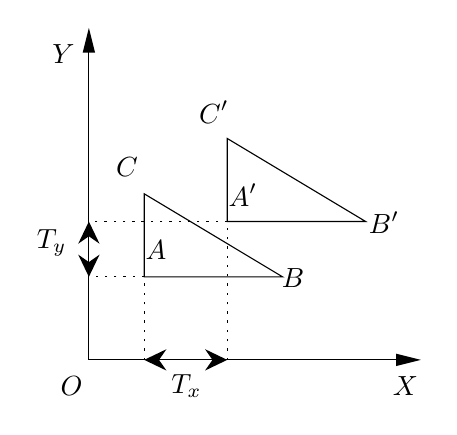
\begin{tikzpicture}[x=0.75pt,y=0.75pt,yscale=-1,xscale=1]
%uncomment if require: \path (0,310); %set diagram left start at 0, and has height of 310

%Straight Lines [id:da0744643818390529] 
\draw    (160,160) -- (160,133.33) -- (160,106.67) -- (160,80) -- (160,53.33) -- (160,26.67) -- (160,2) ;
\draw [shift={(160,0)}, rotate = 90] [fill={rgb, 255:red, 0; green, 0; blue, 0 }  ][line width=0.08]  [draw opacity=0] (12,-3) -- (0,0) -- (12,3) -- cycle    ;
%Straight Lines [id:da2501910192394292] 
\draw    (160,160) -- (186.67,160) -- (213.33,160) -- (240,160) -- (266.67,160) -- (293.33,160) -- (318,160) ;
\draw [shift={(320,160)}, rotate = 180] [fill={rgb, 255:red, 0; green, 0; blue, 0 }  ][line width=0.08]  [draw opacity=0] (12,-3) -- (0,0) -- (12,3) -- cycle    ;
%Shape: Right Triangle [id:dp3230440420217635] 
\draw   (186.67,80) -- (253.33,120) -- (186.67,120) -- cycle ;
%Straight Lines [id:da4274444095380905] 
\draw  [dash pattern={on 0.84pt off 2.51pt}]  (186.67,120) -- (160,120) ;
%Shape: Right Triangle [id:dp3554215710083837] 
\draw   (226.67,53.33) -- (293.33,93.33) -- (226.67,93.33) -- cycle ;
%Straight Lines [id:da18015886667211856] 
\draw  [dash pattern={on 0.84pt off 2.51pt}]  (226.67,93.33) -- (160,93.33) ;
%Straight Lines [id:da20825596809464475] 
\draw  [dash pattern={on 0.84pt off 2.51pt}]  (186.67,160) -- (186.67,137.12) -- (186.67,120) ;
%Straight Lines [id:da30415316219723487] 
\draw  [dash pattern={on 0.84pt off 2.51pt}]  (226.67,160) -- (226.67,93.33) ;
%Straight Lines [id:da18553363748469254] 
\draw    (189.67,160) -- (223.67,160) ;
\draw [shift={(226.67,160)}, rotate = 180] [fill={rgb, 255:red, 0; green, 0; blue, 0 }  ][line width=0.08]  [draw opacity=0] (10.72,-5.15) -- (0,0) -- (10.72,5.15) -- (7.12,0) -- cycle    ;
\draw [shift={(186.67,160)}, rotate = 0] [fill={rgb, 255:red, 0; green, 0; blue, 0 }  ][line width=0.08]  [draw opacity=0] (10.72,-5.15) -- (0,0) -- (10.72,5.15) -- (7.12,0) -- cycle    ;
%Straight Lines [id:da7758481926901326] 
\draw    (160,96.33) -- (160,117) ;
\draw [shift={(160,120)}, rotate = 270] [fill={rgb, 255:red, 0; green, 0; blue, 0 }  ][line width=0.08]  [draw opacity=0] (10.72,-5.15) -- (0,0) -- (10.72,5.15) -- (7.12,0) -- cycle    ;
\draw [shift={(160,93.33)}, rotate = 90] [fill={rgb, 255:red, 0; green, 0; blue, 0 }  ][line width=0.08]  [draw opacity=0] (10.72,-5.15) -- (0,0) -- (10.72,5.15) -- (7.12,0) -- cycle    ;

% Text Node
\draw (312.88,172.78) node   [align=left] {\begin{minipage}[lt]{9.68pt}\setlength\topsep{0pt}
$\displaystyle X$
\end{minipage}};
% Text Node
\draw (150.8,12.78) node   [align=left] {\begin{minipage}[lt]{12.51pt}\setlength\topsep{0pt}
$\displaystyle Y$
\end{minipage}};
% Text Node
\draw (152.88,172.78) node   [align=left] {\begin{minipage}[lt]{9.68pt}\setlength\topsep{0pt}
$\displaystyle O$
\end{minipage}};
% Text Node
\draw (193.79,107.22) node   [align=left] {\begin{minipage}[lt]{9.68pt}\setlength\topsep{0pt}
$\displaystyle A$
\end{minipage}};
% Text Node
\draw (233.79,80.55) node   [align=left] {\begin{minipage}[lt]{9.68pt}\setlength\topsep{0pt}
$\displaystyle A'$
\end{minipage}};
% Text Node
\draw (258.71,120.4) node   [align=left] {\begin{minipage}[lt]{8.67pt}\setlength\topsep{0pt}
$\displaystyle B$
\end{minipage}};
% Text Node
\draw (300.71,94) node   [align=left] {\begin{minipage}[lt]{8.67pt}\setlength\topsep{0pt}
$\displaystyle B'$
\end{minipage}};
% Text Node
\draw (179.55,67.22) node   [align=left] {\begin{minipage}[lt]{9.68pt}\setlength\topsep{0pt}
$\displaystyle C$
\end{minipage}};
% Text Node
\draw (219.55,40.55) node   [align=left] {\begin{minipage}[lt]{9.68pt}\setlength\topsep{0pt}
$\displaystyle C'$
\end{minipage}};
% Text Node
\draw (206.21,172.78) node   [align=left] {\begin{minipage}[lt]{9.68pt}\setlength\topsep{0pt}
$\displaystyle T_{x}$
\end{minipage}};
% Text Node
\draw (141.41,103.58) node   [align=left] {\begin{minipage}[lt]{9.68pt}\setlength\topsep{0pt}
$\displaystyle T_{y}$
\end{minipage}};


\end{tikzpicture}

    }
    \subfigure[scale=.9][比例系数 $S_x=S_y=1$]{
        

\tikzset{every picture/.style={line width=0.75pt}} %set default line width to 0.75pt        

\begin{tikzpicture}[x=0.75pt,y=0.75pt,yscale=-1,xscale=1]
%uncomment if require: \path (0,310); %set diagram left start at 0, and has height of 310

%Straight Lines [id:da15250042942435282] 
\draw    (160,160) -- (160,133.33) -- (160,106.67) -- (160,80) -- (160,53.33) -- (160,26.67) -- (160,2) ;
\draw [shift={(160,0)}, rotate = 90] [fill={rgb, 255:red, 0; green, 0; blue, 0 }  ][line width=0.08]  [draw opacity=0] (12,-3) -- (0,0) -- (12,3) -- cycle    ;
%Straight Lines [id:da8576603280236559] 
\draw    (160,160) -- (186.67,160) -- (213.33,160) -- (240,160) -- (266.67,160) -- (293.33,160) -- (318,160) ;
\draw [shift={(320,160)}, rotate = 180] [fill={rgb, 255:red, 0; green, 0; blue, 0 }  ][line width=0.08]  [draw opacity=0] (12,-3) -- (0,0) -- (12,3) -- cycle    ;
%Shape: Right Triangle [id:dp7502598031763401] 
\draw   (186.67,80) -- (253.33,120) -- (186.67,120) -- cycle ;

% Text Node
\draw (312.88,172.78) node   [align=left] {\begin{minipage}[lt]{9.68pt}\setlength\topsep{0pt}
$\displaystyle X$
\end{minipage}};
% Text Node
\draw (150.8,12.78) node   [align=left] {\begin{minipage}[lt]{12.51pt}\setlength\topsep{0pt}
$\displaystyle Y$
\end{minipage}};
% Text Node
\draw (152.88,172.78) node   [align=left] {\begin{minipage}[lt]{9.68pt}\setlength\topsep{0pt}
$\displaystyle O$
\end{minipage}};
% Text Node
\draw (178.21,107.22) node   [align=left] {\begin{minipage}[lt]{11.5pt}\setlength\topsep{0pt}
$\displaystyle A$
\end{minipage}};
% Text Node
\draw (193.79,107.22) node   [align=left] {\begin{minipage}[lt]{9.68pt}\setlength\topsep{0pt}
$\displaystyle A'$
\end{minipage}};
% Text Node
\draw (247.59,132.78) node   [align=left] {\begin{minipage}[lt]{8.67pt}\setlength\topsep{0pt}
$\displaystyle B$
\end{minipage}};
% Text Node
\draw (259.08,132.78) node   [align=left] {\begin{minipage}[lt]{8.67pt}\setlength\topsep{0pt}
$\displaystyle B'$
\end{minipage}};
% Text Node
\draw (179.55,67.22) node   [align=left] {\begin{minipage}[lt]{9.68pt}\setlength\topsep{0pt}
$\displaystyle C$
\end{minipage}};
% Text Node
\draw (193.79,67.22) node   [align=left] {\begin{minipage}[lt]{9.68pt}\setlength\topsep{0pt}
$\displaystyle C'$
\end{minipage}};


\end{tikzpicture}
    }
    \subfigure[scale=.9][比例系数 $S_x=S_y>1$]{
        

\tikzset{every picture/.style={line width=0.75pt}} %set default line width to 0.75pt        

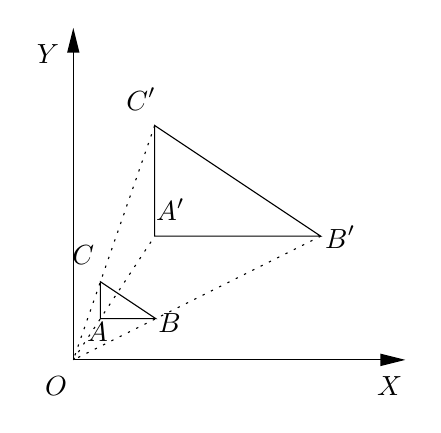
\begin{tikzpicture}[x=0.75pt,y=0.75pt,yscale=-1,xscale=1]
%uncomment if require: \path (0,310); %set diagram left start at 0, and has height of 310

%Straight Lines [id:da1534328502257163] 
\draw    (160,160) -- (160,133.33) -- (160,106.67) -- (160,80) -- (160,53.33) -- (160,26.67) -- (160,2) ;
\draw [shift={(160,0)}, rotate = 90] [fill={rgb, 255:red, 0; green, 0; blue, 0 }  ][line width=0.08]  [draw opacity=0] (12,-3) -- (0,0) -- (12,3) -- cycle    ;
%Straight Lines [id:da05091810398310703] 
\draw    (160,160) -- (186.67,160) -- (213.33,160) -- (240,160) -- (266.67,160) -- (293.33,160) -- (318,160) ;
\draw [shift={(320,160)}, rotate = 180] [fill={rgb, 255:red, 0; green, 0; blue, 0 }  ][line width=0.08]  [draw opacity=0] (12,-3) -- (0,0) -- (12,3) -- cycle    ;
%Shape: Right Triangle [id:dp7699621838177173] 
\draw   (199.2,47.07) -- (279.2,100.4) -- (199.2,100.4) -- cycle ;
%Shape: Right Triangle [id:dp6819256437414682] 
\draw   (173.07,122.36) -- (199.73,140.13) -- (173.07,140.13) -- cycle ;
%Straight Lines [id:da5214539639167379] 
\draw  [dash pattern={on 0.84pt off 2.51pt}]  (199.2,47.07) -- (192.67,65.89) -- (186.13,84.71) -- (179.6,103.53) -- (173.07,122.36) -- (166.53,141.18) -- (160,160) ;
%Straight Lines [id:da8425910163250174] 
\draw  [dash pattern={on 0.84pt off 2.51pt}]  (279.2,100.4) -- (259.33,110.33) -- (239.47,120.27) -- (219.6,130.2) -- (199.73,140.13) -- (179.87,150.07) -- (160,160) ;
%Straight Lines [id:da47875893336700104] 
\draw  [dash pattern={on 0.84pt off 2.51pt}]  (160,160) -- (199.2,100.4) ;

% Text Node
\draw (312.88,172.78) node   [align=left] {\begin{minipage}[lt]{9.68pt}\setlength\topsep{0pt}
$\displaystyle X$
\end{minipage}};
% Text Node
\draw (150.8,12.78) node   [align=left] {\begin{minipage}[lt]{12.51pt}\setlength\topsep{0pt}
$\displaystyle Y$
\end{minipage}};
% Text Node
\draw (152.88,172.78) node   [align=left] {\begin{minipage}[lt]{9.68pt}\setlength\topsep{0pt}
$\displaystyle O$
\end{minipage}};
% Text Node
\draw (173.12,146.42) node   [align=left] {\begin{minipage}[lt]{9.68pt}\setlength\topsep{0pt}
$\displaystyle A$
\end{minipage}};
% Text Node
\draw (206.32,87.62) node   [align=left] {\begin{minipage}[lt]{9.68pt}\setlength\topsep{0pt}
$\displaystyle A'$
\end{minipage}};
% Text Node
\draw (206.71,142.4) node   [align=left] {\begin{minipage}[lt]{8.67pt}\setlength\topsep{0pt}
$\displaystyle B$
\end{minipage}};
% Text Node
\draw (287.11,100.8) node   [align=left] {\begin{minipage}[lt]{8.67pt}\setlength\topsep{0pt}
$\displaystyle B'$
\end{minipage}};
% Text Node
\draw (165.95,109.58) node   [align=left] {\begin{minipage}[lt]{9.68pt}\setlength\topsep{0pt}
$\displaystyle C$
\end{minipage}};
% Text Node
\draw (192.08,34.29) node   [align=left] {\begin{minipage}[lt]{9.68pt}\setlength\topsep{0pt}
$\displaystyle C'$
\end{minipage}};


\end{tikzpicture}

    }
    \subfigure[scale=.9][比例系数 $0<S_x=S_y<1$]{
        

\tikzset{every picture/.style={line width=0.75pt}} %set default line width to 0.75pt        

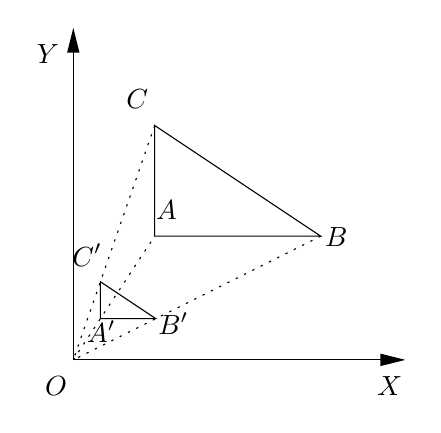
\begin{tikzpicture}[x=0.75pt,y=0.75pt,yscale=-1,xscale=1]
%uncomment if require: \path (0,310); %set diagram left start at 0, and has height of 310

%Straight Lines [id:da9243963150205441] 
\draw    (160,160) -- (160,133.33) -- (160,106.67) -- (160,80) -- (160,53.33) -- (160,26.67) -- (160,2) ;
\draw [shift={(160,0)}, rotate = 90] [fill={rgb, 255:red, 0; green, 0; blue, 0 }  ][line width=0.08]  [draw opacity=0] (12,-3) -- (0,0) -- (12,3) -- cycle    ;
%Straight Lines [id:da8002028753633985] 
\draw    (160,160) -- (186.67,160) -- (213.33,160) -- (240,160) -- (266.67,160) -- (293.33,160) -- (318,160) ;
\draw [shift={(320,160)}, rotate = 180] [fill={rgb, 255:red, 0; green, 0; blue, 0 }  ][line width=0.08]  [draw opacity=0] (12,-3) -- (0,0) -- (12,3) -- cycle    ;
%Shape: Right Triangle [id:dp3074265042318134] 
\draw   (199.2,47.07) -- (279.2,100.4) -- (199.2,100.4) -- cycle ;
%Shape: Right Triangle [id:dp29770002438414234] 
\draw   (173.07,122.36) -- (199.73,140.13) -- (173.07,140.13) -- cycle ;
%Straight Lines [id:da024412753399659648] 
\draw  [dash pattern={on 0.84pt off 2.51pt}]  (199.2,47.07) -- (192.67,65.89) -- (186.13,84.71) -- (179.6,103.53) -- (173.07,122.36) -- (166.53,141.18) -- (160,160) ;
%Straight Lines [id:da7095636127854406] 
\draw  [dash pattern={on 0.84pt off 2.51pt}]  (279.2,100.4) -- (259.33,110.33) -- (239.47,120.27) -- (219.6,130.2) -- (199.73,140.13) -- (179.87,150.07) -- (160,160) ;
%Straight Lines [id:da5652492210181941] 
\draw  [dash pattern={on 0.84pt off 2.51pt}]  (160,160) -- (199.2,100.4) ;

% Text Node
\draw (312.88,172.78) node   [align=left] {\begin{minipage}[lt]{9.68pt}\setlength\topsep{0pt}
$\displaystyle X$
\end{minipage}};
% Text Node
\draw (150.8,12.78) node   [align=left] {\begin{minipage}[lt]{12.51pt}\setlength\topsep{0pt}
$\displaystyle Y$
\end{minipage}};
% Text Node
\draw (152.88,172.78) node   [align=left] {\begin{minipage}[lt]{9.68pt}\setlength\topsep{0pt}
$\displaystyle O$
\end{minipage}};
% Text Node
\draw (173.12,146.42) node   [align=left] {\begin{minipage}[lt]{9.68pt}\setlength\topsep{0pt}
$\displaystyle A'$
\end{minipage}};
% Text Node
\draw (206.32,87.62) node   [align=left] {\begin{minipage}[lt]{9.68pt}\setlength\topsep{0pt}
$\displaystyle A$
\end{minipage}};
% Text Node
\draw (206.71,142.4) node   [align=left] {\begin{minipage}[lt]{8.67pt}\setlength\topsep{0pt}
$\displaystyle B'$
\end{minipage}};
% Text Node
\draw (287.11,100.8) node   [align=left] {\begin{minipage}[lt]{8.67pt}\setlength\topsep{0pt}
$\displaystyle B$
\end{minipage}};
% Text Node
\draw (165.95,109.58) node   [align=left] {\begin{minipage}[lt]{9.68pt}\setlength\topsep{0pt}
$\displaystyle C'$
\end{minipage}};
% Text Node
\draw (192.08,34.29) node   [align=left] {\begin{minipage}[lt]{9.68pt}\setlength\topsep{0pt}
$\displaystyle C$
\end{minipage}};


\end{tikzpicture}

    }
    \subfigure[scale=.9][$S_x=1,~S_y>1$]{
        

\tikzset{every picture/.style={line width=0.75pt}} %set default line width to 0.75pt        

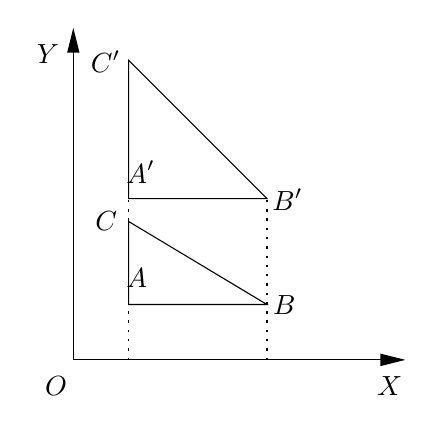
\begin{tikzpicture}[x=0.75pt,y=0.75pt,yscale=-1,xscale=1]
%uncomment if require: \path (0,310); %set diagram left start at 0, and has height of 310

%Straight Lines [id:da8557514491265967] 
\draw    (160,160) -- (160,133.33) -- (160,106.67) -- (160,80) -- (160,53.33) -- (160,26.67) -- (160,2) ;
\draw [shift={(160,0)}, rotate = 90] [fill={rgb, 255:red, 0; green, 0; blue, 0 }  ][line width=0.08]  [draw opacity=0] (12,-3) -- (0,0) -- (12,3) -- cycle    ;
%Straight Lines [id:da5539450143531788] 
\draw    (160,160) -- (186.67,160) -- (213.33,160) -- (240,160) -- (266.67,160) -- (293.33,160) -- (318,160) ;
\draw [shift={(320,160)}, rotate = 180] [fill={rgb, 255:red, 0; green, 0; blue, 0 }  ][line width=0.08]  [draw opacity=0] (12,-3) -- (0,0) -- (12,3) -- cycle    ;
%Straight Lines [id:da5193682179432797] 
\draw  [dash pattern={on 0.84pt off 2.51pt}]  (186.67,160) -- (186.67,82.33) ;
%Shape: Right Triangle [id:dp8688230494789257] 
\draw   (186.67,93.33) -- (253.33,133.33) -- (186.67,133.33) -- cycle ;
%Shape: Right Triangle [id:dp373344497154698] 
\draw   (186.67,15.67) -- (253.33,82.33) -- (186.67,82.33) -- cycle ;
%Straight Lines [id:da7747623883965025] 
\draw  [dash pattern={on 0.84pt off 2.51pt}]  (253.33,160) -- (253.33,82.33) ;

% Text Node
\draw (312.88,172.78) node   [align=left] {\begin{minipage}[lt]{9.68pt}\setlength\topsep{0pt}
$\displaystyle X$
\end{minipage}};
% Text Node
\draw (150.8,12.78) node   [align=left] {\begin{minipage}[lt]{12.51pt}\setlength\topsep{0pt}
$\displaystyle Y$
\end{minipage}};
% Text Node
\draw (152.88,172.78) node   [align=left] {\begin{minipage}[lt]{9.68pt}\setlength\topsep{0pt}
$\displaystyle O$
\end{minipage}};
% Text Node
\draw (191.4,69.55) node   [align=left] {\begin{minipage}[lt]{8.67pt}\setlength\topsep{0pt}
$\displaystyle A'$
\end{minipage}};
% Text Node
\draw (191.4,120.55) node   [align=left] {\begin{minipage}[lt]{8.67pt}\setlength\topsep{0pt}
$\displaystyle A$
\end{minipage}};
% Text Node
\draw (261.71,82.73) node   [align=left] {\begin{minipage}[lt]{8.67pt}\setlength\topsep{0pt}
$\displaystyle B'$
\end{minipage}};
% Text Node
\draw (262.11,133.47) node   [align=left] {\begin{minipage}[lt]{8.67pt}\setlength\topsep{0pt}
$\displaystyle B$
\end{minipage}};
% Text Node
\draw (174.95,16.24) node   [align=left] {\begin{minipage}[lt]{9.68pt}\setlength\topsep{0pt}
$\displaystyle C'$
\end{minipage}};
% Text Node
\draw (177.08,92.95) node   [align=left] {\begin{minipage}[lt]{9.68pt}\setlength\topsep{0pt}
$\displaystyle C$
\end{minipage}};


\end{tikzpicture}

    }
    \subfigure[scale=.9][$Y$ 轴对称]{
        

\tikzset{every picture/.style={line width=0.75pt}} %set default line width to 0.75pt        

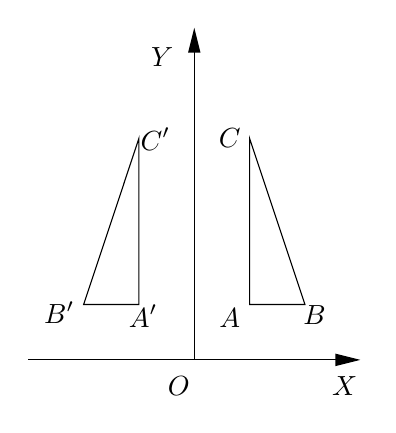
\begin{tikzpicture}[x=0.75pt,y=0.75pt,yscale=-1,xscale=1]
%uncomment if require: \path (0,310); %set diagram left start at 0, and has height of 310

%Straight Lines [id:da9473706495657213] 
\draw    (240,160) -- (240,133.33) -- (240,106.67) -- (240,80) -- (240,53.33) -- (240,26.67) -- (240,2) ;
\draw [shift={(240,0)}, rotate = 90] [fill={rgb, 255:red, 0; green, 0; blue, 0 }  ][line width=0.08]  [draw opacity=0] (12,-3) -- (0,0) -- (12,3) -- cycle    ;
%Straight Lines [id:da3401945044692589] 
\draw    (160,160) -- (186.67,160) -- (213.33,160) -- (240,160) -- (266.67,160) -- (293.33,160) -- (318,160) ;
\draw [shift={(320,160)}, rotate = 180] [fill={rgb, 255:red, 0; green, 0; blue, 0 }  ][line width=0.08]  [draw opacity=0] (12,-3) -- (0,0) -- (12,3) -- cycle    ;
%Shape: Right Triangle [id:dp2883900535142023] 
\draw   (266.67,53.33) -- (293.33,133.33) -- (266.67,133.33) -- cycle ;
%Shape: Right Triangle [id:dp0361672463144318] 
\draw   (213.33,53.33) -- (186.67,133.33) -- (213.33,133.33) -- cycle ;

% Text Node
\draw (312.88,172.78) node   [align=left] {\begin{minipage}[lt]{9.68pt}\setlength\topsep{0pt}
$\displaystyle X$
\end{minipage}};
% Text Node
\draw (227.6,13.98) node   [align=left] {\begin{minipage}[lt]{12.51pt}\setlength\topsep{0pt}
$\displaystyle Y$
\end{minipage}};
% Text Node
\draw (233.79,172.78) node   [align=left] {\begin{minipage}[lt]{9.68pt}\setlength\topsep{0pt}
$\displaystyle O$
\end{minipage}};
% Text Node
\draw (259.81,139.62) node   [align=left] {\begin{minipage}[lt]{11.5pt}\setlength\topsep{0pt}
$\displaystyle A$
\end{minipage}};
% Text Node
\draw (214.99,138.82) node   [align=left] {\begin{minipage}[lt]{9.68pt}\setlength\topsep{0pt}
$\displaystyle A'$
\end{minipage}};
% Text Node
\draw (298.39,138.38) node   [align=left] {\begin{minipage}[lt]{8.67pt}\setlength\topsep{0pt}
$\displaystyle B$
\end{minipage}};
% Text Node
\draw (173.48,137.18) node   [align=left] {\begin{minipage}[lt]{8.67pt}\setlength\topsep{0pt}
$\displaystyle B'$
\end{minipage}};
% Text Node
\draw (258.35,53.22) node   [align=left] {\begin{minipage}[lt]{9.68pt}\setlength\topsep{0pt}
$\displaystyle C$
\end{minipage}};
% Text Node
\draw (220.59,53.62) node   [align=left] {\begin{minipage}[lt]{9.68pt}\setlength\topsep{0pt}
$\displaystyle C'$
\end{minipage}};


\end{tikzpicture}

    }
    \subfigure[scale=.9][$X$ 轴对称]{
        

\tikzset{every picture/.style={line width=0.75pt}} %set default line width to 0.75pt        

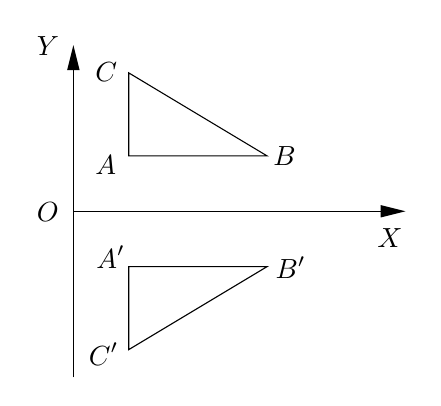
\begin{tikzpicture}[x=0.75pt,y=0.75pt,yscale=-1,xscale=1]
%uncomment if require: \path (0,310); %set diagram left start at 0, and has height of 310

%Straight Lines [id:da24368355678437692] 
\draw    (160,240) -- (160,213.33) -- (160,186.67) -- (160,160) -- (160,133.33) -- (160,106.67) -- (160,82) ;
\draw [shift={(160,80)}, rotate = 90] [fill={rgb, 255:red, 0; green, 0; blue, 0 }  ][line width=0.08]  [draw opacity=0] (12,-3) -- (0,0) -- (12,3) -- cycle    ;
%Straight Lines [id:da91989606623083] 
\draw    (160,160) -- (186.67,160) -- (213.33,160) -- (240,160) -- (266.67,160) -- (293.33,160) -- (318,160) ;
\draw [shift={(320,160)}, rotate = 180] [fill={rgb, 255:red, 0; green, 0; blue, 0 }  ][line width=0.08]  [draw opacity=0] (12,-3) -- (0,0) -- (12,3) -- cycle    ;
%Shape: Right Triangle [id:dp6047665119381709] 
\draw   (186.67,93.33) -- (253.33,133.33) -- (186.67,133.33) -- cycle ;
%Shape: Right Triangle [id:dp2085112249426042] 
\draw   (186.67,226.67) -- (253.33,186.67) -- (186.67,186.67) -- cycle ;

% Text Node
\draw (312.88,172.78) node   [align=left] {\begin{minipage}[lt]{9.68pt}\setlength\topsep{0pt}
$\displaystyle X$
\end{minipage}};
% Text Node
\draw (150.8,80.55) node   [align=left] {\begin{minipage}[lt]{12.51pt}\setlength\topsep{0pt}
$\displaystyle Y$
\end{minipage}};
% Text Node
\draw (148.88,160.28) node   [align=left] {\begin{minipage}[lt]{9.68pt}\setlength\topsep{0pt}
$\displaystyle O$
\end{minipage}};
% Text Node
\draw (176.9,182.05) node   [align=left] {\begin{minipage}[lt]{8.67pt}\setlength\topsep{0pt}
$\displaystyle A'$
\end{minipage}};
% Text Node
\draw (176.4,137.55) node   [align=left] {\begin{minipage}[lt]{8.67pt}\setlength\topsep{0pt}
$\displaystyle A$
\end{minipage}};
% Text Node
\draw (263.21,187.23) node   [align=left] {\begin{minipage}[lt]{8.67pt}\setlength\topsep{0pt}
$\displaystyle B'$
\end{minipage}};
% Text Node
\draw (262.11,133.47) node   [align=left] {\begin{minipage}[lt]{8.67pt}\setlength\topsep{0pt}
$\displaystyle B$
\end{minipage}};
% Text Node
\draw (173.95,228.74) node   [align=left] {\begin{minipage}[lt]{9.68pt}\setlength\topsep{0pt}
$\displaystyle C'$
\end{minipage}};
% Text Node
\draw (177.08,92.95) node   [align=left] {\begin{minipage}[lt]{9.68pt}\setlength\topsep{0pt}
$\displaystyle C$
\end{minipage}};


\end{tikzpicture}

    }
    \subfigure[scale=.9][中心对称]{
        

\tikzset{every picture/.style={line width=0.75pt}} %set default line width to 0.75pt        

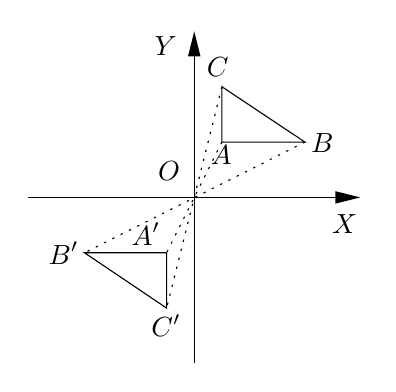
\begin{tikzpicture}[x=0.75pt,y=0.75pt,yscale=-1,xscale=1]
%uncomment if require: \path (0,310); %set diagram left start at 0, and has height of 310

%Straight Lines [id:da20466553477334037] 
\draw    (240,240) -- (240,213.33) -- (240,186.67) -- (240,160) -- (240,133.33) -- (240,106.67) -- (240,82) ;
\draw [shift={(240,80)}, rotate = 90] [fill={rgb, 255:red, 0; green, 0; blue, 0 }  ][line width=0.08]  [draw opacity=0] (12,-3) -- (0,0) -- (12,3) -- cycle    ;
%Straight Lines [id:da07906371106904819] 
\draw    (160,160) -- (186.67,160) -- (213.33,160) -- (240,160) -- (266.67,160) -- (293.33,160) -- (318,160) ;
\draw [shift={(320,160)}, rotate = 180] [fill={rgb, 255:red, 0; green, 0; blue, 0 }  ][line width=0.08]  [draw opacity=0] (12,-3) -- (0,0) -- (12,3) -- cycle    ;
%Shape: Right Triangle [id:dp711098921084359] 
\draw   (253.33,106.67) -- (293.33,133.33) -- (253.33,133.33) -- cycle ;
%Shape: Right Triangle [id:dp32855978989430157] 
\draw   (226.67,213.33) -- (187.13,186.67) -- (226.67,186.67) -- cycle ;
%Straight Lines [id:da813083554485903] 
\draw  [dash pattern={on 0.84pt off 2.51pt}]  (253.33,133.33) -- (226.67,186.67) ;
%Straight Lines [id:da3857126514317757] 
\draw  [dash pattern={on 0.84pt off 2.51pt}]  (293.33,133.33) -- (187.13,186.67) ;
%Straight Lines [id:da811525310685079] 
\draw  [dash pattern={on 0.84pt off 2.51pt}]  (253.33,106.67) -- (226.67,213.33) ;

% Text Node
\draw (312.88,172.78) node   [align=left] {\begin{minipage}[lt]{9.68pt}\setlength\topsep{0pt}
$\displaystyle X$
\end{minipage}};
% Text Node
\draw (229.2,87.22) node   [align=left] {\begin{minipage}[lt]{12.51pt}\setlength\topsep{0pt}
$\displaystyle Y$
\end{minipage}};
% Text Node
\draw (230.85,147.22) node   [align=left] {\begin{minipage}[lt]{12.44pt}\setlength\topsep{0pt}
$\displaystyle O$
\end{minipage}};
% Text Node
\draw (255.71,139.72) node   [align=left] {\begin{minipage}[lt]{11.5pt}\setlength\topsep{0pt}
$\displaystyle A$
\end{minipage}};
% Text Node
\draw (216.29,177.72) node   [align=left] {\begin{minipage}[lt]{9.68pt}\setlength\topsep{0pt}
$\displaystyle A'$
\end{minipage}};
% Text Node
\draw (302.09,133.78) node   [align=left] {\begin{minipage}[lt]{8.67pt}\setlength\topsep{0pt}
$\displaystyle B$
\end{minipage}};
% Text Node
\draw (175.58,186.78) node   [align=left] {\begin{minipage}[lt]{8.67pt}\setlength\topsep{0pt}
$\displaystyle B'$
\end{minipage}};
% Text Node
\draw (252.55,97.22) node   [align=left] {\begin{minipage}[lt]{9.68pt}\setlength\topsep{0pt}
$\displaystyle C$
\end{minipage}};
% Text Node
\draw (225.79,221.72) node   [align=left] {\begin{minipage}[lt]{9.68pt}\setlength\topsep{0pt}
$\displaystyle C'$
\end{minipage}};


\end{tikzpicture}

    }
    \subfigure[scale=.9][$Y=X$ 对称]{
        

\tikzset{every picture/.style={line width=0.75pt}} %set default line width to 0.75pt        

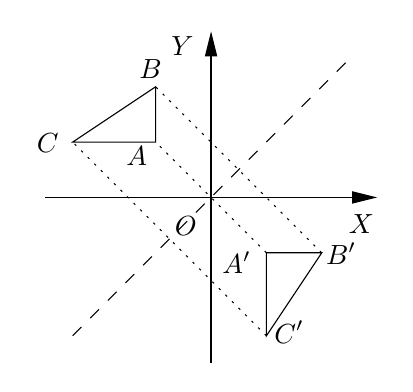
\begin{tikzpicture}[x=0.75pt,y=0.75pt,yscale=-1,xscale=1]
%uncomment if require: \path (0,310); %set diagram left start at 0, and has height of 310

%Straight Lines [id:da8292659722722793] 
\draw    (240,240) -- (240,213.33) -- (240,186.67) -- (240,160) -- (240,133.33) -- (240,106.67) -- (240,82) ;
\draw [shift={(240,80)}, rotate = 90] [fill={rgb, 255:red, 0; green, 0; blue, 0 }  ][line width=0.08]  [draw opacity=0] (12,-3) -- (0,0) -- (12,3) -- cycle    ;
%Straight Lines [id:da7352149228464684] 
\draw    (160,160) -- (186.67,160) -- (213.33,160) -- (240,160) -- (266.67,160) -- (293.33,160) -- (318,160) ;
\draw [shift={(320,160)}, rotate = 180] [fill={rgb, 255:red, 0; green, 0; blue, 0 }  ][line width=0.08]  [draw opacity=0] (12,-3) -- (0,0) -- (12,3) -- cycle    ;
%Straight Lines [id:da2661475178458712] 
\draw  [dash pattern={on 0.84pt off 2.51pt}]  (266.67,186.67) -- (213.33,133.33) ;
%Shape: Right Triangle [id:dp6596390866394817] 
\draw   (213.33,106.67) -- (173.33,133.33) -- (213.33,133.33) -- cycle ;
%Straight Lines [id:da7951069745564614] 
\draw  [dash pattern={on 4.5pt off 4.5pt}]  (173.33,226.67) -- (306.67,93.33) ;
%Shape: Right Triangle [id:dp32508442712015806] 
\draw   (266.67,226.67) -- (293.33,186.67) -- (266.67,186.67) -- cycle ;
%Straight Lines [id:da9943714913243453] 
\draw  [dash pattern={on 0.84pt off 2.51pt}]  (293.33,186.67) -- (213.33,106.67) ;
%Straight Lines [id:da42142200377858186] 
\draw  [dash pattern={on 0.84pt off 2.51pt}]  (266.67,226.67) -- (173.33,133.33) ;

% Text Node
\draw (312.88,172.78) node   [align=left] {\begin{minipage}[lt]{9.68pt}\setlength\topsep{0pt}
$\displaystyle X$
\end{minipage}};
% Text Node
\draw (229.2,87.22) node   [align=left] {\begin{minipage}[lt]{12.51pt}\setlength\topsep{0pt}
$\displaystyle Y$
\end{minipage}};
% Text Node
\draw (230.85,173.89) node   [align=left] {\begin{minipage}[lt]{12.44pt}\setlength\topsep{0pt}
$\displaystyle O$
\end{minipage}};
% Text Node
\draw (206.91,140.12) node   [align=left] {\begin{minipage}[lt]{11.5pt}\setlength\topsep{0pt}
$\displaystyle A$
\end{minipage}};
% Text Node
\draw (251.89,191.32) node   [align=left] {\begin{minipage}[lt]{9.68pt}\setlength\topsep{0pt}
$\displaystyle A'$
\end{minipage}};
% Text Node
\draw (211.29,98.18) node   [align=left] {\begin{minipage}[lt]{8.67pt}\setlength\topsep{0pt}
$\displaystyle B$
\end{minipage}};
% Text Node
\draw (301.18,187.18) node   [align=left] {\begin{minipage}[lt]{8.67pt}\setlength\topsep{0pt}
$\displaystyle B'$
\end{minipage}};
% Text Node
\draw (162.55,134.02) node   [align=left] {\begin{minipage}[lt]{9.68pt}\setlength\topsep{0pt}
$\displaystyle C$
\end{minipage}};
% Text Node
\draw (276.99,224.92) node   [align=left] {\begin{minipage}[lt]{9.68pt}\setlength\topsep{0pt}
$\displaystyle C'$
\end{minipage}};


\end{tikzpicture}

    }
    \subfigure[scale=.9][$Y=-X$ 对称]{
        

\tikzset{every picture/.style={line width=0.75pt}} %set default line width to 0.75pt        

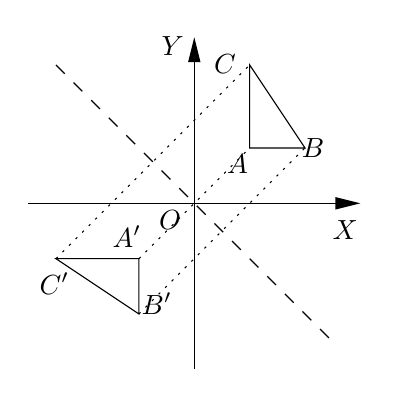
\begin{tikzpicture}[x=0.75pt,y=0.75pt,yscale=-1,xscale=1]
%uncomment if require: \path (0,310); %set diagram left start at 0, and has height of 310

%Straight Lines [id:da2266867895070097] 
\draw    (155.13,159.59) -- (181.8,159.59) -- (208.47,159.59) -- (235.13,159.59) -- (261.8,159.59) -- (288.47,159.59) -- (313.13,159.59) ;
\draw [shift={(315.13,159.59)}, rotate = 180] [fill={rgb, 255:red, 0; green, 0; blue, 0 }  ][line width=0.08]  [draw opacity=0] (12,-3) -- (0,0) -- (12,3) -- cycle    ;
%Straight Lines [id:da4885018729597703] 
\draw    (235.13,81.59) -- (235.13,106.25) -- (235.13,132.92) -- (235.13,159.59) -- (235.13,186.25) -- (235.13,212.92) -- (235.13,239.59) ;
\draw [shift={(235.13,79.59)}, rotate = 90] [fill={rgb, 255:red, 0; green, 0; blue, 0 }  ][line width=0.08]  [draw opacity=0] (12,-3) -- (0,0) -- (12,3) -- cycle    ;
%Straight Lines [id:da37798418466605876] 
\draw  [dash pattern={on 0.84pt off 2.51pt}]  (208.47,186.25) -- (261.8,132.92) ;
%Shape: Right Triangle [id:dp9937709437984665] 
\draw   (288.47,132.92) -- (261.8,92.92) -- (261.8,132.92) -- cycle ;
%Straight Lines [id:da8376057486917463] 
\draw  [dash pattern={on 4.5pt off 4.5pt}]  (168.47,92.92) -- (301.8,226.25) ;
%Shape: Right Triangle [id:dp15886819391939877] 
\draw   (168.47,186.25) -- (208.47,212.92) -- (208.47,186.25) -- cycle ;
%Straight Lines [id:da8724202073941834] 
\draw  [dash pattern={on 0.84pt off 2.51pt}]  (208.47,212.92) -- (288.47,132.92) ;
%Straight Lines [id:da8687627509248148] 
\draw  [dash pattern={on 0.84pt off 2.51pt}]  (168.47,186.25) -- (261.8,92.92) ;

% Text Node
\draw (307.55,172.37) node   [align=left] {\begin{minipage}[lt]{8.67pt}\setlength\topsep{0pt}
$\displaystyle X$
\end{minipage}};
% Text Node
\draw (225.15,83.97) node   [align=left] {\begin{minipage}[lt]{8.67pt}\setlength\topsep{0pt}
$\displaystyle Y$
\end{minipage}};
% Text Node
\draw (223.95,167.57) node   [align=left] {\begin{minipage}[lt]{8.67pt}\setlength\topsep{0pt}
$\displaystyle O$
\end{minipage}};
% Text Node
\draw (256.75,140.77) node   [align=left] {\begin{minipage}[lt]{8.67pt}\setlength\topsep{0pt}
$\displaystyle A$
\end{minipage}};
% Text Node
\draw (201.55,175.57) node   [align=left] {\begin{minipage}[lt]{8.67pt}\setlength\topsep{0pt}
$\displaystyle A'$
\end{minipage}};
% Text Node
\draw (292.75,133.17) node   [align=left] {\begin{minipage}[lt]{8.67pt}\setlength\topsep{0pt}
$\displaystyle B$
\end{minipage}};
% Text Node
\draw (250.45,92.54) node   [align=left] {\begin{minipage}[lt]{8.67pt}\setlength\topsep{0pt}
$\displaystyle C$
\end{minipage}};
% Text Node
\draw (215.55,207.97) node   [align=left] {\begin{minipage}[lt]{8.67pt}\setlength\topsep{0pt}
$\displaystyle B'$
\end{minipage}};
% Text Node
\draw (166.35,198.37) node   [align=left] {\begin{minipage}[lt]{8.67pt}\setlength\topsep{0pt}
$\displaystyle C'$
\end{minipage}};


\end{tikzpicture}

    }
    \subfigure[scale=.9][相对原点旋转 $\theta$ 角]{
        

\tikzset{every picture/.style={line width=0.75pt}} %set default line width to 0.75pt        

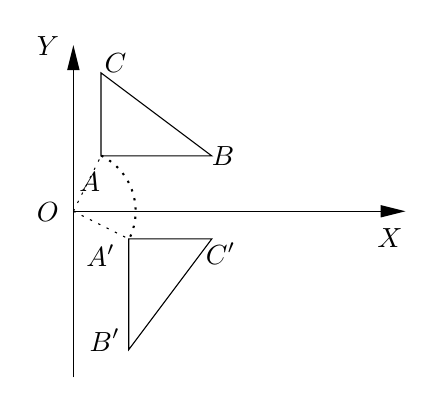
\begin{tikzpicture}[x=0.75pt,y=0.75pt,yscale=-1,xscale=1]
%uncomment if require: \path (0,310); %set diagram left start at 0, and has height of 310

%Straight Lines [id:da713951749740587] 
\draw    (160,240) -- (160,213.33) -- (160,186.67) -- (160,160) -- (160,133.33) -- (160,106.67) -- (160,82) ;
\draw [shift={(160,80)}, rotate = 90] [fill={rgb, 255:red, 0; green, 0; blue, 0 }  ][line width=0.08]  [draw opacity=0] (12,-3) -- (0,0) -- (12,3) -- cycle    ;
%Straight Lines [id:da27505852441502276] 
\draw    (160,160) -- (186.67,160) -- (213.33,160) -- (240,160) -- (266.67,160) -- (293.33,160) -- (318,160) ;
\draw [shift={(320,160)}, rotate = 180] [fill={rgb, 255:red, 0; green, 0; blue, 0 }  ][line width=0.08]  [draw opacity=0] (12,-3) -- (0,0) -- (12,3) -- cycle    ;
%Shape: Right Triangle [id:dp9653910433627337] 
\draw   (173.33,93.33) -- (226.67,133.33) -- (173.33,133.33) -- cycle ;
%Shape: Right Triangle [id:dp19153562200662932] 
\draw   (226.67,173.33) -- (186.67,226.67) -- (186.67,173.33) -- cycle ;
%Straight Lines [id:da6181416799790123] 
\draw  [dash pattern={on 0.84pt off 2.51pt}]  (160,160) -- (173.33,133.33) ;
%Straight Lines [id:da34341147568550356] 
\draw  [dash pattern={on 0.84pt off 2.51pt}]  (160,160) -- (186.67,173.33) ;
%Shape: Arc [id:dp3703274603787783] 
\draw  [draw opacity=0][dash pattern={on 0.84pt off 2.51pt}][line width=0.75]  (173.45,133.18) .. controls (183.26,138.11) and (190,148.27) .. (190,160) .. controls (190,164.85) and (188.85,169.43) .. (186.81,173.48) -- (160,160) -- cycle ; \draw  [dash pattern={on 0.84pt off 2.51pt}][line width=0.75]  (173.45,133.18) .. controls (183.26,138.11) and (190,148.27) .. (190,160) .. controls (190,164.85) and (188.85,169.43) .. (186.81,173.48) ;  

% Text Node
\draw (312.88,172.78) node   [align=left] {\begin{minipage}[lt]{9.68pt}\setlength\topsep{0pt}
$\displaystyle X$
\end{minipage}};
% Text Node
\draw (150.8,80.55) node   [align=left] {\begin{minipage}[lt]{12.51pt}\setlength\topsep{0pt}
$\displaystyle Y$
\end{minipage}};
% Text Node
\draw (148.88,160.28) node   [align=left] {\begin{minipage}[lt]{9.68pt}\setlength\topsep{0pt}
$\displaystyle O$
\end{minipage}};
% Text Node
\draw (172.1,181.25) node   [align=left] {\begin{minipage}[lt]{8.67pt}\setlength\topsep{0pt}
$\displaystyle A'$
\end{minipage}};
% Text Node
\draw (168.72,145.96) node   [align=left] {\begin{minipage}[lt]{8.67pt}\setlength\topsep{0pt}
$\displaystyle A$
\end{minipage}};
% Text Node
\draw (173.61,222.03) node   [align=left] {\begin{minipage}[lt]{8.67pt}\setlength\topsep{0pt}
$\displaystyle B'$
\end{minipage}};
% Text Node
\draw (232.51,133.47) node   [align=left] {\begin{minipage}[lt]{8.67pt}\setlength\topsep{0pt}
$\displaystyle B$
\end{minipage}};
% Text Node
\draw (230.35,180.34) node   [align=left] {\begin{minipage}[lt]{9.68pt}\setlength\topsep{0pt}
$\displaystyle C'$
\end{minipage}};
% Text Node
\draw (181.48,88.55) node   [align=left] {\begin{minipage}[lt]{9.68pt}\setlength\topsep{0pt}
$\displaystyle C$
\end{minipage}};


\end{tikzpicture}

    }
    \subfigure[scale=.9][$X$ 方向错切]{
        

\tikzset{every picture/.style={line width=0.75pt}} %set default line width to 0.75pt        

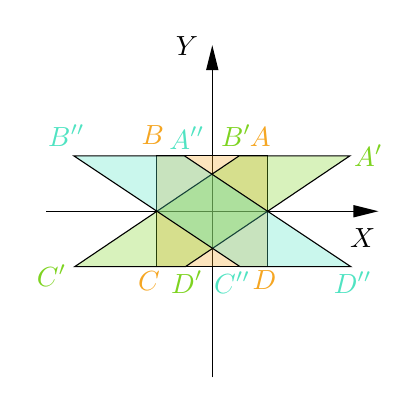
\begin{tikzpicture}[x=0.75pt,y=0.75pt,yscale=-1,xscale=1]
%uncomment if require: \path (0,310); %set diagram left start at 0, and has height of 310

%Straight Lines [id:da258215525060401] 
\draw    (240,240) -- (240,213.33) -- (240,186.67) -- (240,160) -- (240,133.33) -- (240,106.67) -- (240,82) ;
\draw [shift={(240,80)}, rotate = 90] [fill={rgb, 255:red, 0; green, 0; blue, 0 }  ][line width=0.08]  [draw opacity=0] (12,-3) -- (0,0) -- (12,3) -- cycle    ;
%Straight Lines [id:da058671601265665174] 
\draw    (160,160) -- (186.67,160) -- (213.33,160) -- (240,160) -- (266.67,160) -- (293.33,160) -- (318,160) ;
\draw [shift={(320,160)}, rotate = 180] [fill={rgb, 255:red, 0; green, 0; blue, 0 }  ][line width=0.08]  [draw opacity=0] (12,-3) -- (0,0) -- (12,3) -- cycle    ;
%Shape: Rectangle [id:dp4811001215484525] 
\draw  [fill={rgb, 255:red, 245; green, 166; blue, 35 }  ,fill opacity=0.3 ] (213.33,133.33) -- (266.67,133.33) -- (266.67,186.67) -- (213.33,186.67) -- cycle ;
%Shape: Rectangle [id:dp8297367285498773] 
\draw  [fill={rgb, 255:red, 126; green, 211; blue, 33 }  ,fill opacity=0.3 ] (252.91,133.33) -- (306.24,133.33) -- (227.09,186.67) -- (173.76,186.67) -- cycle ;
%Shape: Rectangle [id:dp18591382614366458] 
\draw  [fill={rgb, 255:red, 80; green, 227; blue, 194 }  ,fill opacity=0.3 ] (173.31,133.33) -- (226.64,133.33) -- (306.69,186.67) -- (253.36,186.67) -- cycle ;

% Text Node
\draw (312.88,172.78) node   [align=left] {\begin{minipage}[lt]{9.68pt}\setlength\topsep{0pt}
$\displaystyle X$
\end{minipage}};
% Text Node
\draw (230.8,80.55) node   [align=left] {\begin{minipage}[lt]{12.51pt}\setlength\topsep{0pt}
$\displaystyle Y$
\end{minipage}};
% Text Node
\draw (314.1,133.25) node  [color={rgb, 255:red, 126; green, 211; blue, 33 }  ,opacity=1 ] [align=left] {\begin{minipage}[lt]{8.67pt}\setlength\topsep{0pt}
$\displaystyle A'$
\end{minipage}};
% Text Node
\draw (263.92,124.36) node  [color={rgb, 255:red, 245; green, 166; blue, 35 }  ,opacity=1 ] [align=left] {\begin{minipage}[lt]{8.67pt}\setlength\topsep{0pt}
$\displaystyle A$
\end{minipage}};
% Text Node
\draw (250.01,123.63) node  [color={rgb, 255:red, 126; green, 211; blue, 33 }  ,opacity=1 ] [align=left] {\begin{minipage}[lt]{8.67pt}\setlength\topsep{0pt}
$\displaystyle B'$
\end{minipage}};
% Text Node
\draw (211.71,123.47) node  [color={rgb, 255:red, 245; green, 166; blue, 35 }  ,opacity=1 ] [align=left] {\begin{minipage}[lt]{8.67pt}\setlength\topsep{0pt}
$\displaystyle B$
\end{minipage}};
% Text Node
\draw (161.95,191.14) node  [color={rgb, 255:red, 126; green, 211; blue, 33 }  ,opacity=1 ] [align=left] {\begin{minipage}[lt]{9.68pt}\setlength\topsep{0pt}
$\displaystyle C'$
\end{minipage}};
% Text Node
\draw (210.68,193.75) node  [color={rgb, 255:red, 245; green, 166; blue, 35 }  ,opacity=1 ] [align=left] {\begin{minipage}[lt]{9.68pt}\setlength\topsep{0pt}
$\displaystyle C$
\end{minipage}};
% Text Node
\draw (265.88,193.35) node  [color={rgb, 255:red, 245; green, 166; blue, 35 }  ,opacity=1 ] [align=left] {\begin{minipage}[lt]{9.68pt}\setlength\topsep{0pt}
$\displaystyle D$
\end{minipage}};
% Text Node
\draw (226.68,194.15) node  [color={rgb, 255:red, 126; green, 211; blue, 33 }  ,opacity=1 ] [align=left] {\begin{minipage}[lt]{9.68pt}\setlength\topsep{0pt}
$\displaystyle D'$
\end{minipage}};
% Text Node
\draw (225.12,124.76) node  [color={rgb, 255:red, 80; green, 227; blue, 194 }  ,opacity=1 ] [align=left] {\begin{minipage}[lt]{8.67pt}\setlength\topsep{0pt}
$\displaystyle A''$
\end{minipage}};
% Text Node
\draw (166.72,123.56) node  [color={rgb, 255:red, 80; green, 227; blue, 194 }  ,opacity=1 ] [align=left] {\begin{minipage}[lt]{8.67pt}\setlength\topsep{0pt}
$\displaystyle B''$
\end{minipage}};
% Text Node
\draw (246.72,194.36) node  [color={rgb, 255:red, 80; green, 227; blue, 194 }  ,opacity=1 ] [align=left] {\begin{minipage}[lt]{8.67pt}\setlength\topsep{0pt}
$\displaystyle C''$
\end{minipage}};
% Text Node
\draw (304.32,194.36) node  [color={rgb, 255:red, 80; green, 227; blue, 194 }  ,opacity=1 ] [align=left] {\begin{minipage}[lt]{8.67pt}\setlength\topsep{0pt}
$\displaystyle D''$
\end{minipage}};


\end{tikzpicture}

    }
    \caption{}
    \label{jihebh}
\end{figure}